\chapter{User Manual}
\label{usermanual}

% In the user manual you should explain, step-by-step, how to reproduce the demo that you showed in the oral presentation or the results you mentioned in the previous chapters.\\ If it is necessary to install some toolchain that is already well described in the original documentation (i.e., Espressif's toolchain for ESP32 boards or the SEcube toolchain) just insert a reference to the original documentation (and remember to clearly specify which version of the original documentation must be used). There is no need to copy and paste step-by-step guides that are already well-written and available.\\The user manual must explain how to re-create what you did in the project, no matter if it is low-level code (i..e VHDL on SEcube's FPGA), high-level code (i.e., a GUI) or something more heterogeneous (i.e. a bunch of ESP32 or Raspberry Pi communicating among them and interacting with other devices).

\subsection{Firmware}
This tutorial needs a working version of Eclipse for C/C++ and the AC6 Tools are properly installed in order to build the firmware and flash it to the SECube device. The configuration describes uses the following configuration:
\begin{itemize}
	\item ST-Link/v2 programmer
	\item Eclipse IDE for C/C++ Developers (includes Incubating components) Version: 2022-03 (4.23.0) Build id: 20220310-1457
	\item Ubuntu 18.04 5.4.0-117-generic
\end{itemize}

\subsubsection{Hardware and Compiler setup}
In this Section are reported the instructions you need to follow to properly connect the SEcube DevKit to the Host PC and to Programmer/debugger, refer to Figure \ref{fig:setup2}. A more detailed configuration tutorial is available via the  \href{https://github.com/SEcube-Project/SEcube-SDK/blob/master/wiki/wiki_rel_012.pdf}{official SECube Wiki}.

\begin{figure}[H]
	\centering
	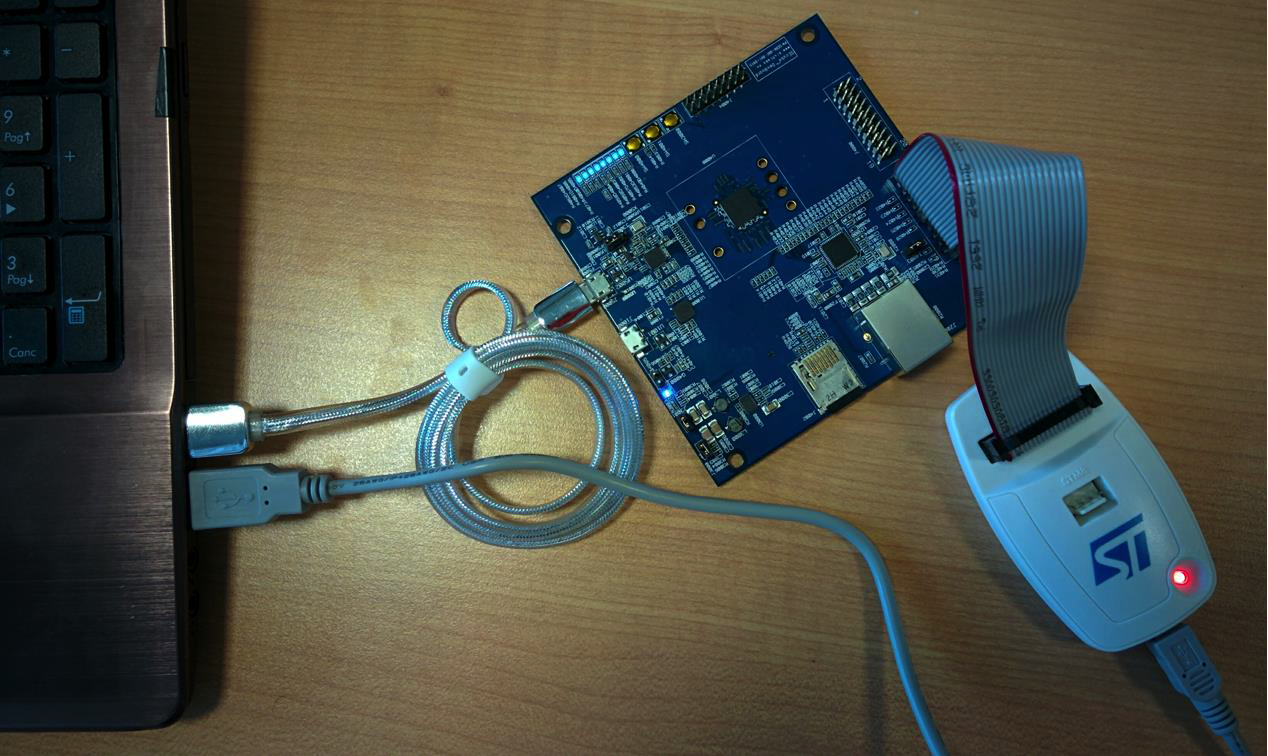
\includegraphics[width=0.42\linewidth]{images/firmware/setup_2}
	\caption{Connection between the STLink/v2 programmer and the SEcube DevKit}
	\label{fig:setup2}
\end{figure}

\begin{figure}
	\centering
	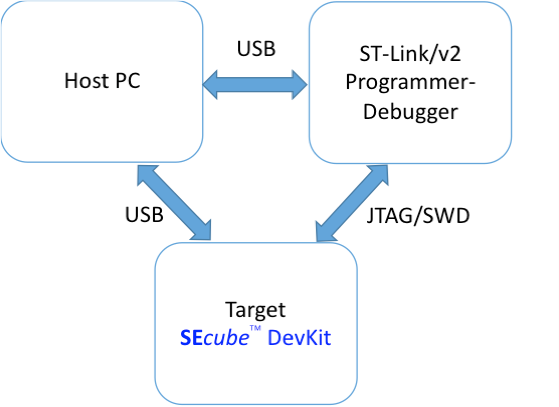
\includegraphics[width=0.35\linewidth]{images/firmware/setup_4}
	\caption{System Architecture}
	\label{fig:setup4}
\end{figure}


Assembling is composed of the following two steps in order to obtain the situation that is available at Figure \ref{fig:setup4}:
\begin{enumerate}
	\item Connect the SEcube DevKit with the programmer by means of the JTAG/SWD cable: the
	      cable should be inserted on the JTAG docks on both the programmer (in this case the orientation of the plug is forced from the dock) and the DevKit (in this case you must pay
	      attention in inserting the plug on top of both lines of connectors and with its protrusion
	      oriented towards the inner side of the DevKit).
	\item Connect the ST-Link/v2 with the PC by means of the USB cable.
\end{enumerate}
The system assembled is shown in Figure \ref{fig:setup2}, while a close-up on the JTAG connection is in Figure \ref{fig:setup3}.

\begin{figure}
	\centering
	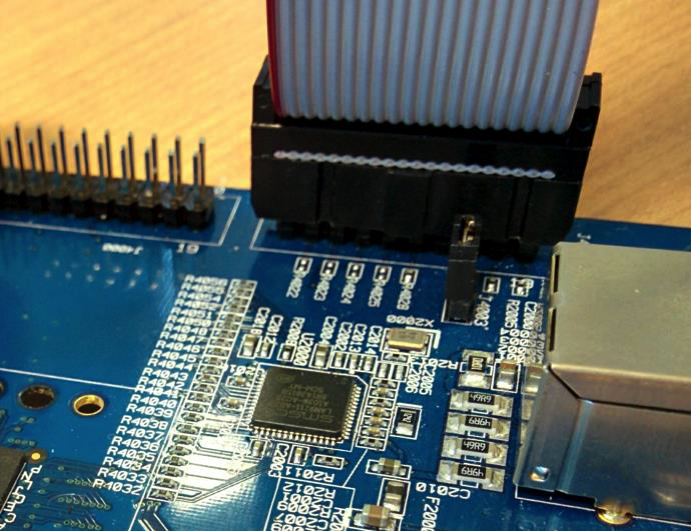
\includegraphics[width=0.35\linewidth]{images/firmware/setup_3}
	\caption{Connection between the STLink/v2 programmer and the SEcubeTM DevKit, close-up (highlighted in red) on the JTAG connector orientation}
	\label{fig:setup3}
\end{figure}


In order to be able to build and flash the firmware, the AC6 Tools must be installed via Eclipse. The AC6 Tool will install the GNU Embedded Toolchain for ARM, which is a ready-to-use, open
source suite of tools for C, C++ and Assembly programming targeting ARM Cortex-M and Cortex-R
family of processors. It includes the GNU Compiler (GCC) and is available free of charge directly
from ARM for embedded so ware development on both Windows and Linux operating systems.
The reference platform for this document is the System Workbench for STM32 (SW4STM32) Eclipse
plugin.

SW4STM32 is an integrated environment that includes:
\begin{itemize}
	\item Building tools (GCC-based ARM cross compiler, assembler and linker);
	\item OpenOCD and GDB debugging tools;
	\item Flash programming tools
\end{itemize}

To install SW4STM32 as an Eclipse plugin:
\begin{enumerate}
	\item launch Eclipse IDE
	\item on the toolbar, click «Help » Install New Software...»
	\item in the Available Software window, click «Add»
	\item in the Add Repository window, set Name and Location fields as follows, and then click «OK»:
	      \begin{itemize}
		      \item Name: System Workbench for STM32 - Bare Machine edition
		      \item Locaton: http://www.ac6-tools.com/Eclipse-updates/org.openstm32.system-workbench.site
	      \end{itemize}
	\item select OpenSTM32 Tools and click «Next»
	\item accept the license agreement and click «Finish» to start the plugin installation, continue the installation also if a warning for incompatible or unsigned components is prompted
	\item restart Eclipse
\end{enumerate}



\subsubsection{Firmware flashing}
Once the SECube has been connected to the Host computer via both the ST-Link/v2 programmer and the USB connection, the firmware can be imported, compiled and flashed.

The latest firmware version has been already compiled and available at ``\textit{SEcube USBStick Firmware/Project/Eclipse/USBStick/Release/USBStick.elf}" but it is possible to import the project into Eclipse and recompile it. If you want to use the pre-compiled version, you can skip the following sections and go to Section \ref{sec:firm_configure}.

In order to import the firmware and the software for performing the init, you need to click «File» and then «Import...», as in Figure \ref{fig:setup6}. At this point after having selected «Existing Projects into Workspace» (Figure \ref{fig:setup7}), the first two projects must be imported (Figure \ref{fig:setup8}).
\begin{figure}[H]
	\centering
	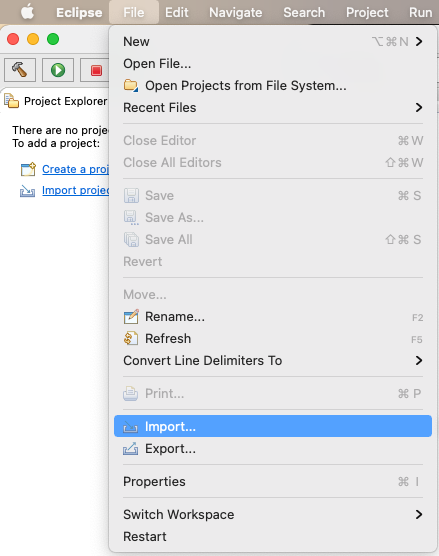
\includegraphics[width=0.45\linewidth]{images/firmware/setup_6}
	\caption{Project import in Eclipse}
	\label{fig:setup6}
\end{figure}
\begin{figure}[H]
	\centering
	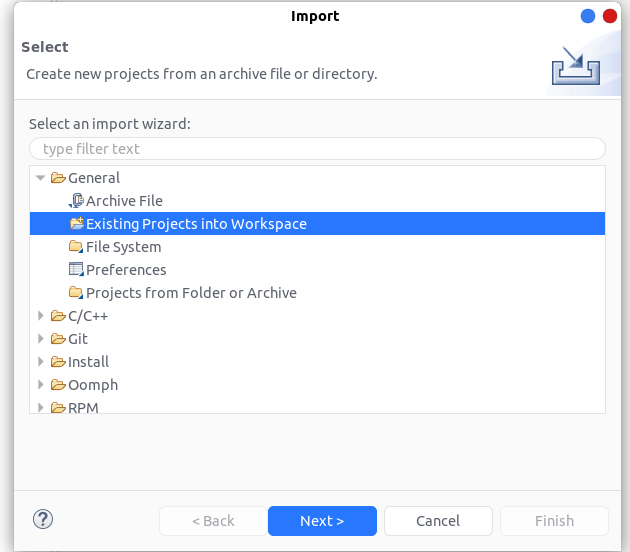
\includegraphics[width=0.6\linewidth]{images/firmware/setup_7}
	\caption{Import of projects}
	\label{fig:setup7}
\end{figure}

\begin{figure}[H]
	\centering
	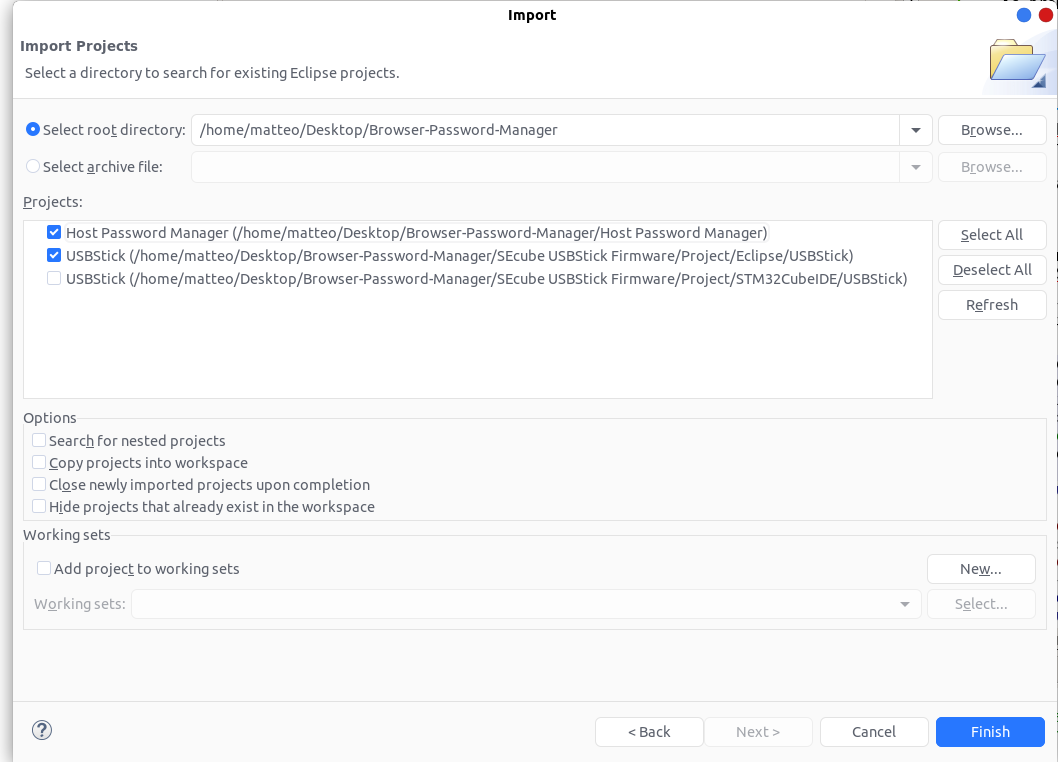
\includegraphics[width=0.6\linewidth]{images/firmware/setup_8}
	\caption{USBStick firmware and Host Password Manager for Initilization}
	\label{fig:setup8}
\end{figure}

The first project will be used during configuration of the device while the second one is the firmware itself.

At this point, on the right you should have two projects, you have to Right click over the ``USBStick" one and select ``Build Project" (refer to Figure \ref{fig:setup10}).
\begin{figure}[H]
	\centering
	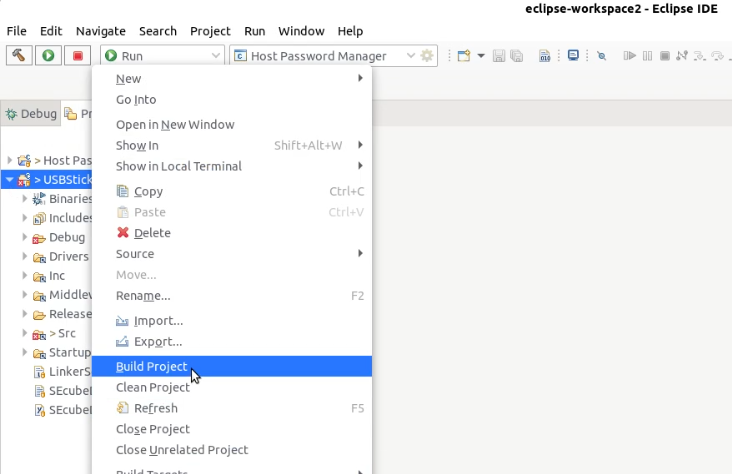
\includegraphics[width=0.55\linewidth]{images/firmware/setup_10}
	\caption{Build the firmware}
	\label{fig:setup10}
\end{figure}

\subsubsection{Configuring the device}
\label{sec:firm_configure}
Once the firmware, you have to first of all to erase the chip in order to remove the previous pin configuration, by doing a Right click on the project and then ``Target" and then ``Erase Chip...". Once it has finished, you can flash the firmware into to the device by clicking ``Target" and then ``Program Chip..." (refer to Figure \ref{fig:setup11}). In the next window you have to select the ``Release" version and flag the ``Reset after program" before clicking ``OK".

\begin{figure}[H]
	\centering
	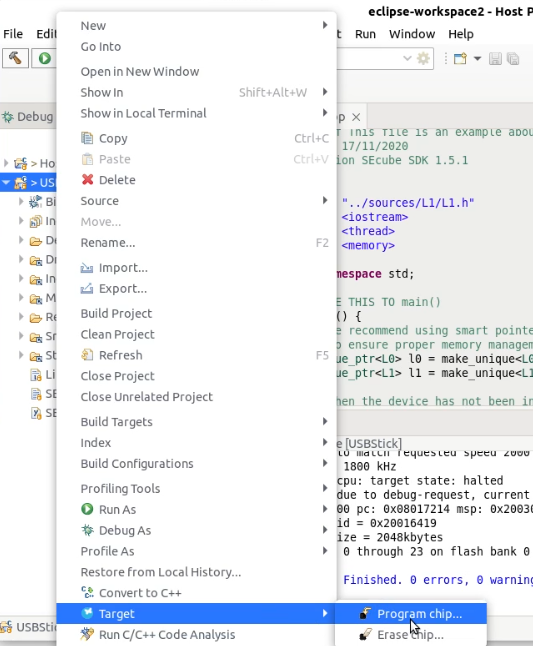
\includegraphics[width=0.55\linewidth]{images/firmware/setup_11}
	\caption{Flash the firmware}
	\label{fig:setup11}
\end{figure}


\begin{figure}[H]
	\centering
	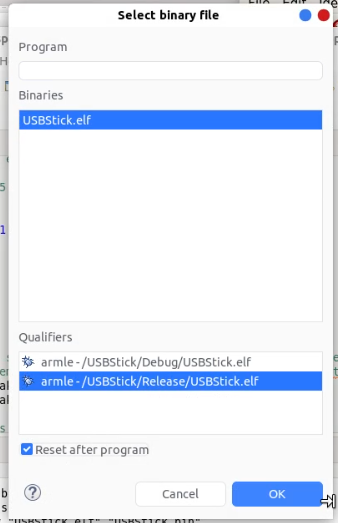
\includegraphics[width=0.3\linewidth]{images/firmware/setup_12}
	\caption{Firmware Release version selection}
	\label{fig:setup12}
\end{figure}

At this point, once the firmware has been flash, you need to configure the device by setting a pin. Now it is the turn of the second project called ``Host Password Manager".\newline\newline
You have to open the \texttt{device\_init.cpp} file and check that the name of the first method is set to \texttt{main}. At this point, you can perform the compilation and run the program. This allows to initialize the device and set the master password for the Secure Password Manager (at line 49 it is possible to change the pin). From now, the device is ready to receive commands by the Host Middleware application in order to manage all passwords features.

\section{Host Middleware}

This section will describe how to build and run the host middleware, both on Linux and Windows. The build process is not necessary because a ready-to-run executable will be provided for the two opearting systems. However, if there are problems in executing them, the build process can be used as a workaround.

\begin{warning}
\textbf{ATTENTION}: because of all the dependencies and operations to perform to achieve a working build, \textbf{many problems may occurr}. This section will try to indicate all the necessary software that are required, but unfortunately the successful build of the host middleware is not guaranteed because of the heterogeneous nature of computers.
\end{warning}

\subsection{Linux}
Luckily, on Linux the build process is pretty straightforward. The only thing that needs to be done is to install the necessary software. The following is a list of software that is required to build the host middleware.

\begin{itemize}
	\item \textbf{Python 3.9.x} (tested with 3.9.7). Check that your PATH environment variable points to the Python executable \textit{python3}.
	\item \textbf{pip 20.3.4} (tested with 20.3.4). Check that your PATH environment variable points to the pip executable \textit{pip} and refers to the correct Python version.
	\item \textbf{gcc 11.x} {tested with 11.2.0}. Check that your PATH environment variable points to the gcc executable \textit{gcc}.
	\item \textbf{g++ 11.x} {tested with 11.2.0}. Check that your PATH environment variable points to the g++ executable \textit{g++}.
	\item \textbf{GNU Make} {tested with GNU Make 4.3}. Check that your PATH environment variable points to the GNU Make executable \textit{make}.
	\item \textbf{git} Check that your PATH environment variable points to the git executable \textit{git}.
\end{itemize}

Here a few steps to build the host middleware if all the required software is installed correctly. Note, it can change depending on the used linux distribution. It may requre further steps to install the dependencies.

\begin{lstlisting}[language=bash,caption={bash version}]
$ git clone https://github.com/SEcube-Project/Browser-Password-Manager.git
$ cd Browser-Password-Manager/HostMiddleware

# To build the shared library
$ make clean
$ make -j4 lib.so

# To run the scrypt as-is (include build of lib.so)
$ make clean
$ make -j4 run

# To compile, obfuscate and pack into a single executable
$ make clean
$ make -j4 dist
$ ./BPMMiddleware

\end{lstlisting}


\subsection{Windows}
Unfortunately, on Windows there is a lot more work to do.

\subsubsection{Python}
Python 3.9.x is needed. If you are not sure it's installed on your system, try to launch a Powershell console and type \texttt{python --version}. If you get \texttt{Python 3.9.0} or similar means that Python is installed. Otherwise, you need to install it. \\

\begin{warning}
\textbf{ATTENTION}: if the Windows Store opens up, close it! You need to install it in the \textit{classic way} otherwise strange things will happens later one. 
\end{warning}

\begin{warning}
\textbf{ATTENTION}: if you installed Python from the Windows Store, unistall and download it from \href{https://www.python.org/downloads/release/python-390/}{the official Python webpage}.
\end{warning}

\begin{warning}
	\textbf{ATTENTION}: if python is not available from the Powershell after manual installation, try to reboot. If it's still not available, you need to manually specify the Python's executable path. Start menù, type Python, right-click and select "Open File location". Most likely it will head you to the Start Menu Shortcuts, so right-click again on the Python 3.9 folder and click on "Open file location". Select the path and copy in the clipboard.

	In the start menu, search for "environment" and click "Edit the system environment variable". Click on "environment variables" button, select "Path", click "Edit", click "New" and paste the path you previously copied.

	Confirm and close everthing, the Powershell too. Open it again and check if now python is available.
\end{warning}

\subsubsection{C++ Compiler - Buildtools}
Head to the start menù and look for \texttt{x64 Native Tools Command Prompt for VS 2022} (if you are on a 32 bit system, look for \texttt{x86 Native Tools Command Prompt for VS 2022}). Open it, and a terminal emulator will show up. Type \texttt{cl}. If you get \textit{'cl' is not recognized as an internal or external program...} means that something is missing, otherwise you will get the following message and it means that the compiler is installed. Same reasoning must undergo with the \texttt{link} command.

\begin{lstlisting}[language=bash,caption={bash version}]
C:\Program Files\Microsoft Visual Studio\2022\Community>cl
Microsoft (R) C/C++ Optimizing Compiler Version 19.32.31329 for x64
Copyright (C) Microsoft Corporation.  All rights reserved.

usage: cl [ option... ] filename... [ /link linkoption... ]

C:\Program Files\Microsoft Visual Studio\2022\Community>link
Microsoft (R) Incremental Linker Version 14.32.31329.0
Copyright (C) Microsoft Corporation.  All rights reserved.

 usage: LINK [options] [files] [@commandfile]

   options:

      /ALIGN:#
      /ALLOWBIND[:NO]
      /ALLOWISOLATION[:NO]
      /APPCONTAINER[:NO]
      /ASSEMBLYDEBUG[:DISABLE]
      /ASSEMBLYLINKRESOURCE:filename
      /ASSEMBLYMODULE:filename
      /ASSEMBLYRESOURCE:filename[,[name][,PRIVATE]]
      /BASE:{address[,size]|@filename,key}
      /CLRIMAGETYPE:{IJW|PURE|SAFE|SAFE32BITPREFERRED}
      /CLRLOADEROPTIMIZATION:{MD|MDH|NONE|SD}
      /CLRSUPPORTLASTERROR[:{NO|SYSTEMDLL}]
      /CLRTHREADATTRIBUTE:{MTA|NONE|STA}
      /CLRUNMANAGEDCODECHECK[:NO]
      /DEBUG[:{FASTLINK|FULL|NONE}]
      /DEF:filename
      /DEFAULTLIB:library
      /DELAY:{NOBIND|UNLOAD}
      /DELAYLOAD:dll
      /DELAYSIGN[:NO]
      /DEPENDENTLOADFLAG:flag
      /DLL
      /DRIVER[:{UPONLY|WDM}]
      /DYNAMICBASE[:NO]
      /EMITVOLATILEMETADATA[:NO]
(press <return> to continue)

\end{lstlisting}

If something is missing (or the Visual Studio's Command Prompt Tool is not available), Visual Studio must be installed. Go to \href{https://visualstudio.microsoft.com/downloads/}{https://visualstudio.microsoft.com/downloads/} and download Visual Studio Community edition. Once the installer is downloaded, launch it, select \textit{Visual Studio Community 2022} (click on Modify if Visual Studio is already installed) and select \textit{Desktop Development with C++}. The following parts must be installed:

\begin{itemize}
	\item MSVC v143 - VS 2022 C++ x64/x86 build Tools
	\item Windows 10 SDK
	\item C++/CLI support for v143 build Tools
	\item C++ Modules for v143 build tools
	\item C++ Clang tools for Windows
\end{itemize}

Repeat from the beginning, be sure that the \textit{Visual Studio's Command Prompt} is installed and the compiler is available.

\subsubsection{How to build}
Now everything should be installed. Open the Visual Studio's Command Prompt, head to the HostMiddleware folder (with the CD command) and type \texttt{compile\_win.bat}. It will compile everything and pack into a single BPMMiddleware.exe executable that eventually you can run, if everything went fine.\\

Pay attention to antivirus software, it may block the executable. If it does, you can try to disable the antivirus temporarily. Pay attention to use the right Visual Studio's Command Prompt version: if you are on a 64 bit system, use \texttt{x64} instead of \texttt{x86}.\\

If there are problems in packing the executable, you can always try to run directly the python code as-is (under the condition that the dll has been compiled correctly): run \texttt{python app.py}.

\subsection{Extension}

In this section it is described how to build (and eventually modify on your needs) and run the extension. This process is the same on all platforms.
The build process is not necessary because a ready to run extension will be provided.

\subsubsection{Installing dependencies and enabling extension developer mode}
The whole extension is built thanks to node packages. So it is important to install node, following the clear instruction given on the \href{https://nodejs.org/}{Nodejs webpage}.

\begin{warning}
	\textbf{ATTENTION}: it is important to install at least Node \textbf{16.x.x} Using an older version may cause some error building the extension.
\end{warning}
To check the node version, type \texttt{node --version}. 

The next step is to enable the \texttt{Developer mode} in order to able to load the extension to the browser. For these tutorial we will use Google Chrome, but the process is the same on all Chromium based browsers (Microsoft Edge Chromium, Brave etc.. ).

Open the Browser, go to the three vertical dots in the top right corner of the browser, click them, then hover on the \textit{More Tools} menu. A submenu will open, click on \textit{Extensions}.

As shown in the \autoref{fig:developer_mode} below, you will find a toggle button, allowing you to enable or disable the developer mode.

% Add the image
\begin{figure}[htb]
	\centering
	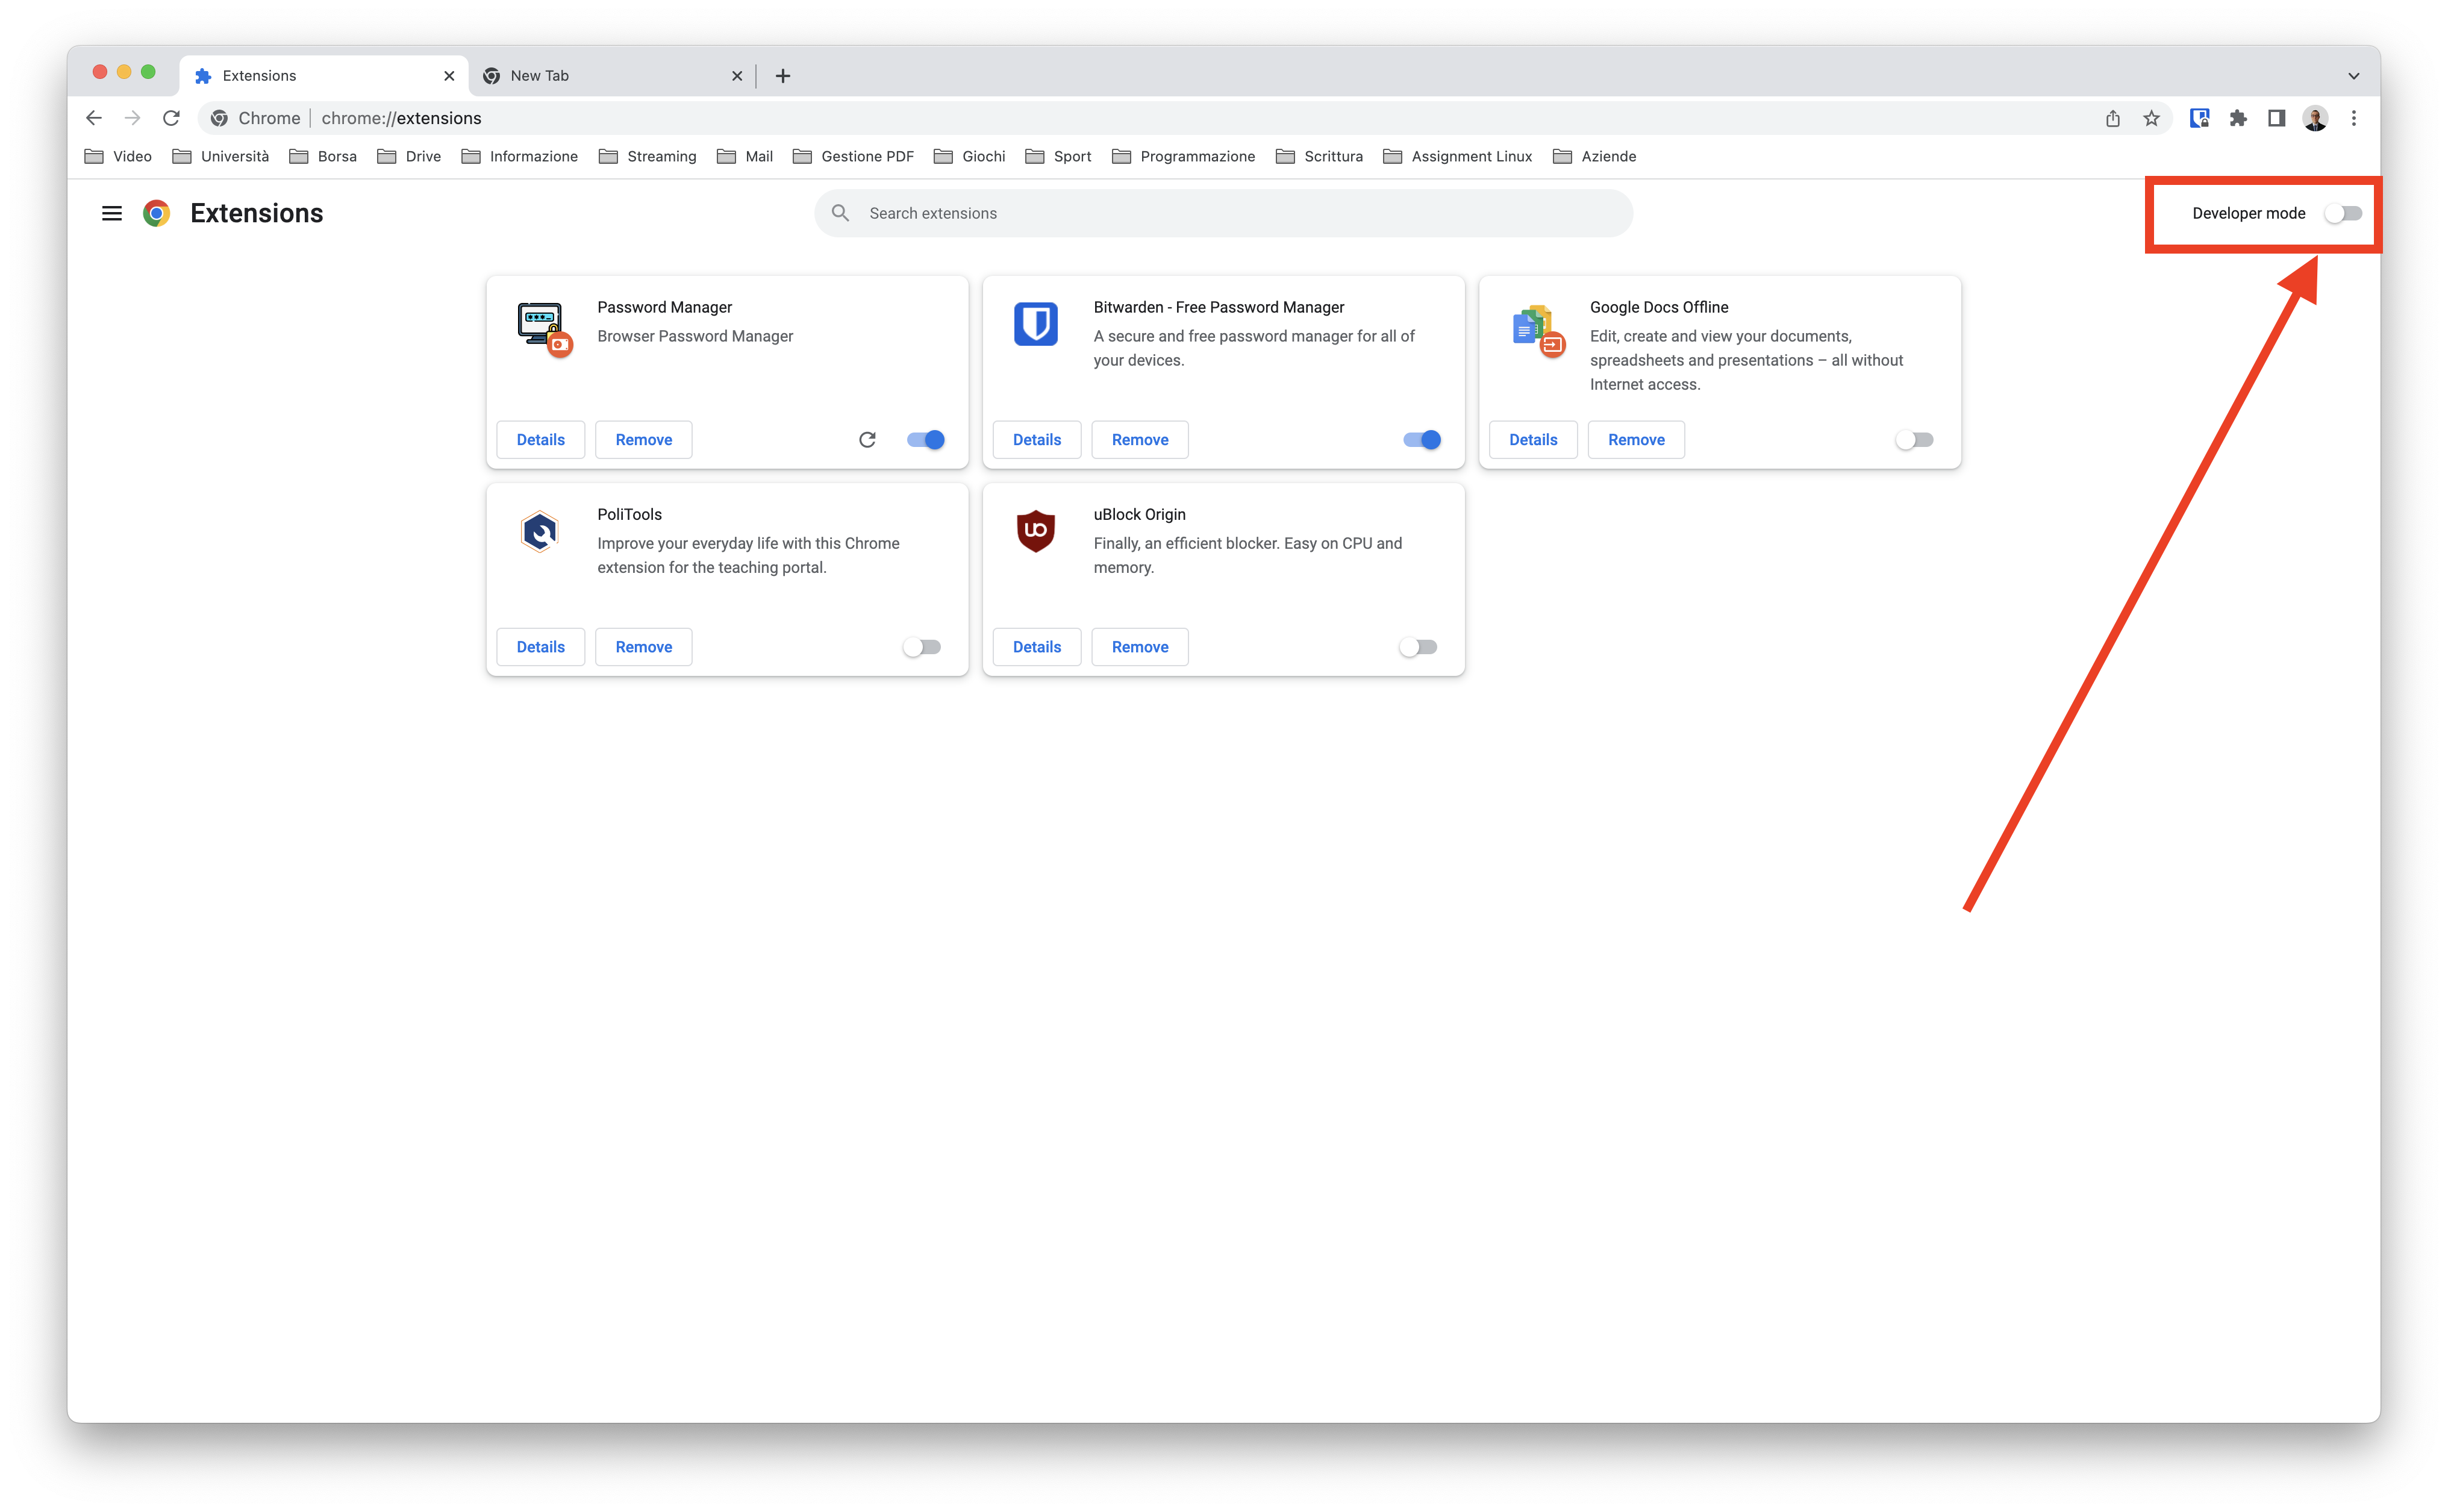
\includegraphics[width=0.8\textwidth]{images/extension/developer-mode.png}
	\caption{Developer mode}
	\label{fig:developer_mode}
\end{figure}

\subsubsection{Build the extension}

Building the extension is very easy. Just open a terminal and go in the \texttt{Chrome Extensions} folder. Type \texttt{npm i} and wait for the installation to finish. With this command all packages are installed. If, for any reason, you want to modify the extension and you need new packages, just add them to the \texttt{package.json} file.
When the installation of the packages is finished you can start building the extension. Type \texttt{npm start} and wait for the build to finish. After this command you will see a new folder called \texttt{dist}.
Now you can go back to the browser and click the button \textbf{Load Unpacked}. A file selection popup will open, to allow the user to select the folder to load.
% Add the image
\begin{figure}[htb]
	\centering
	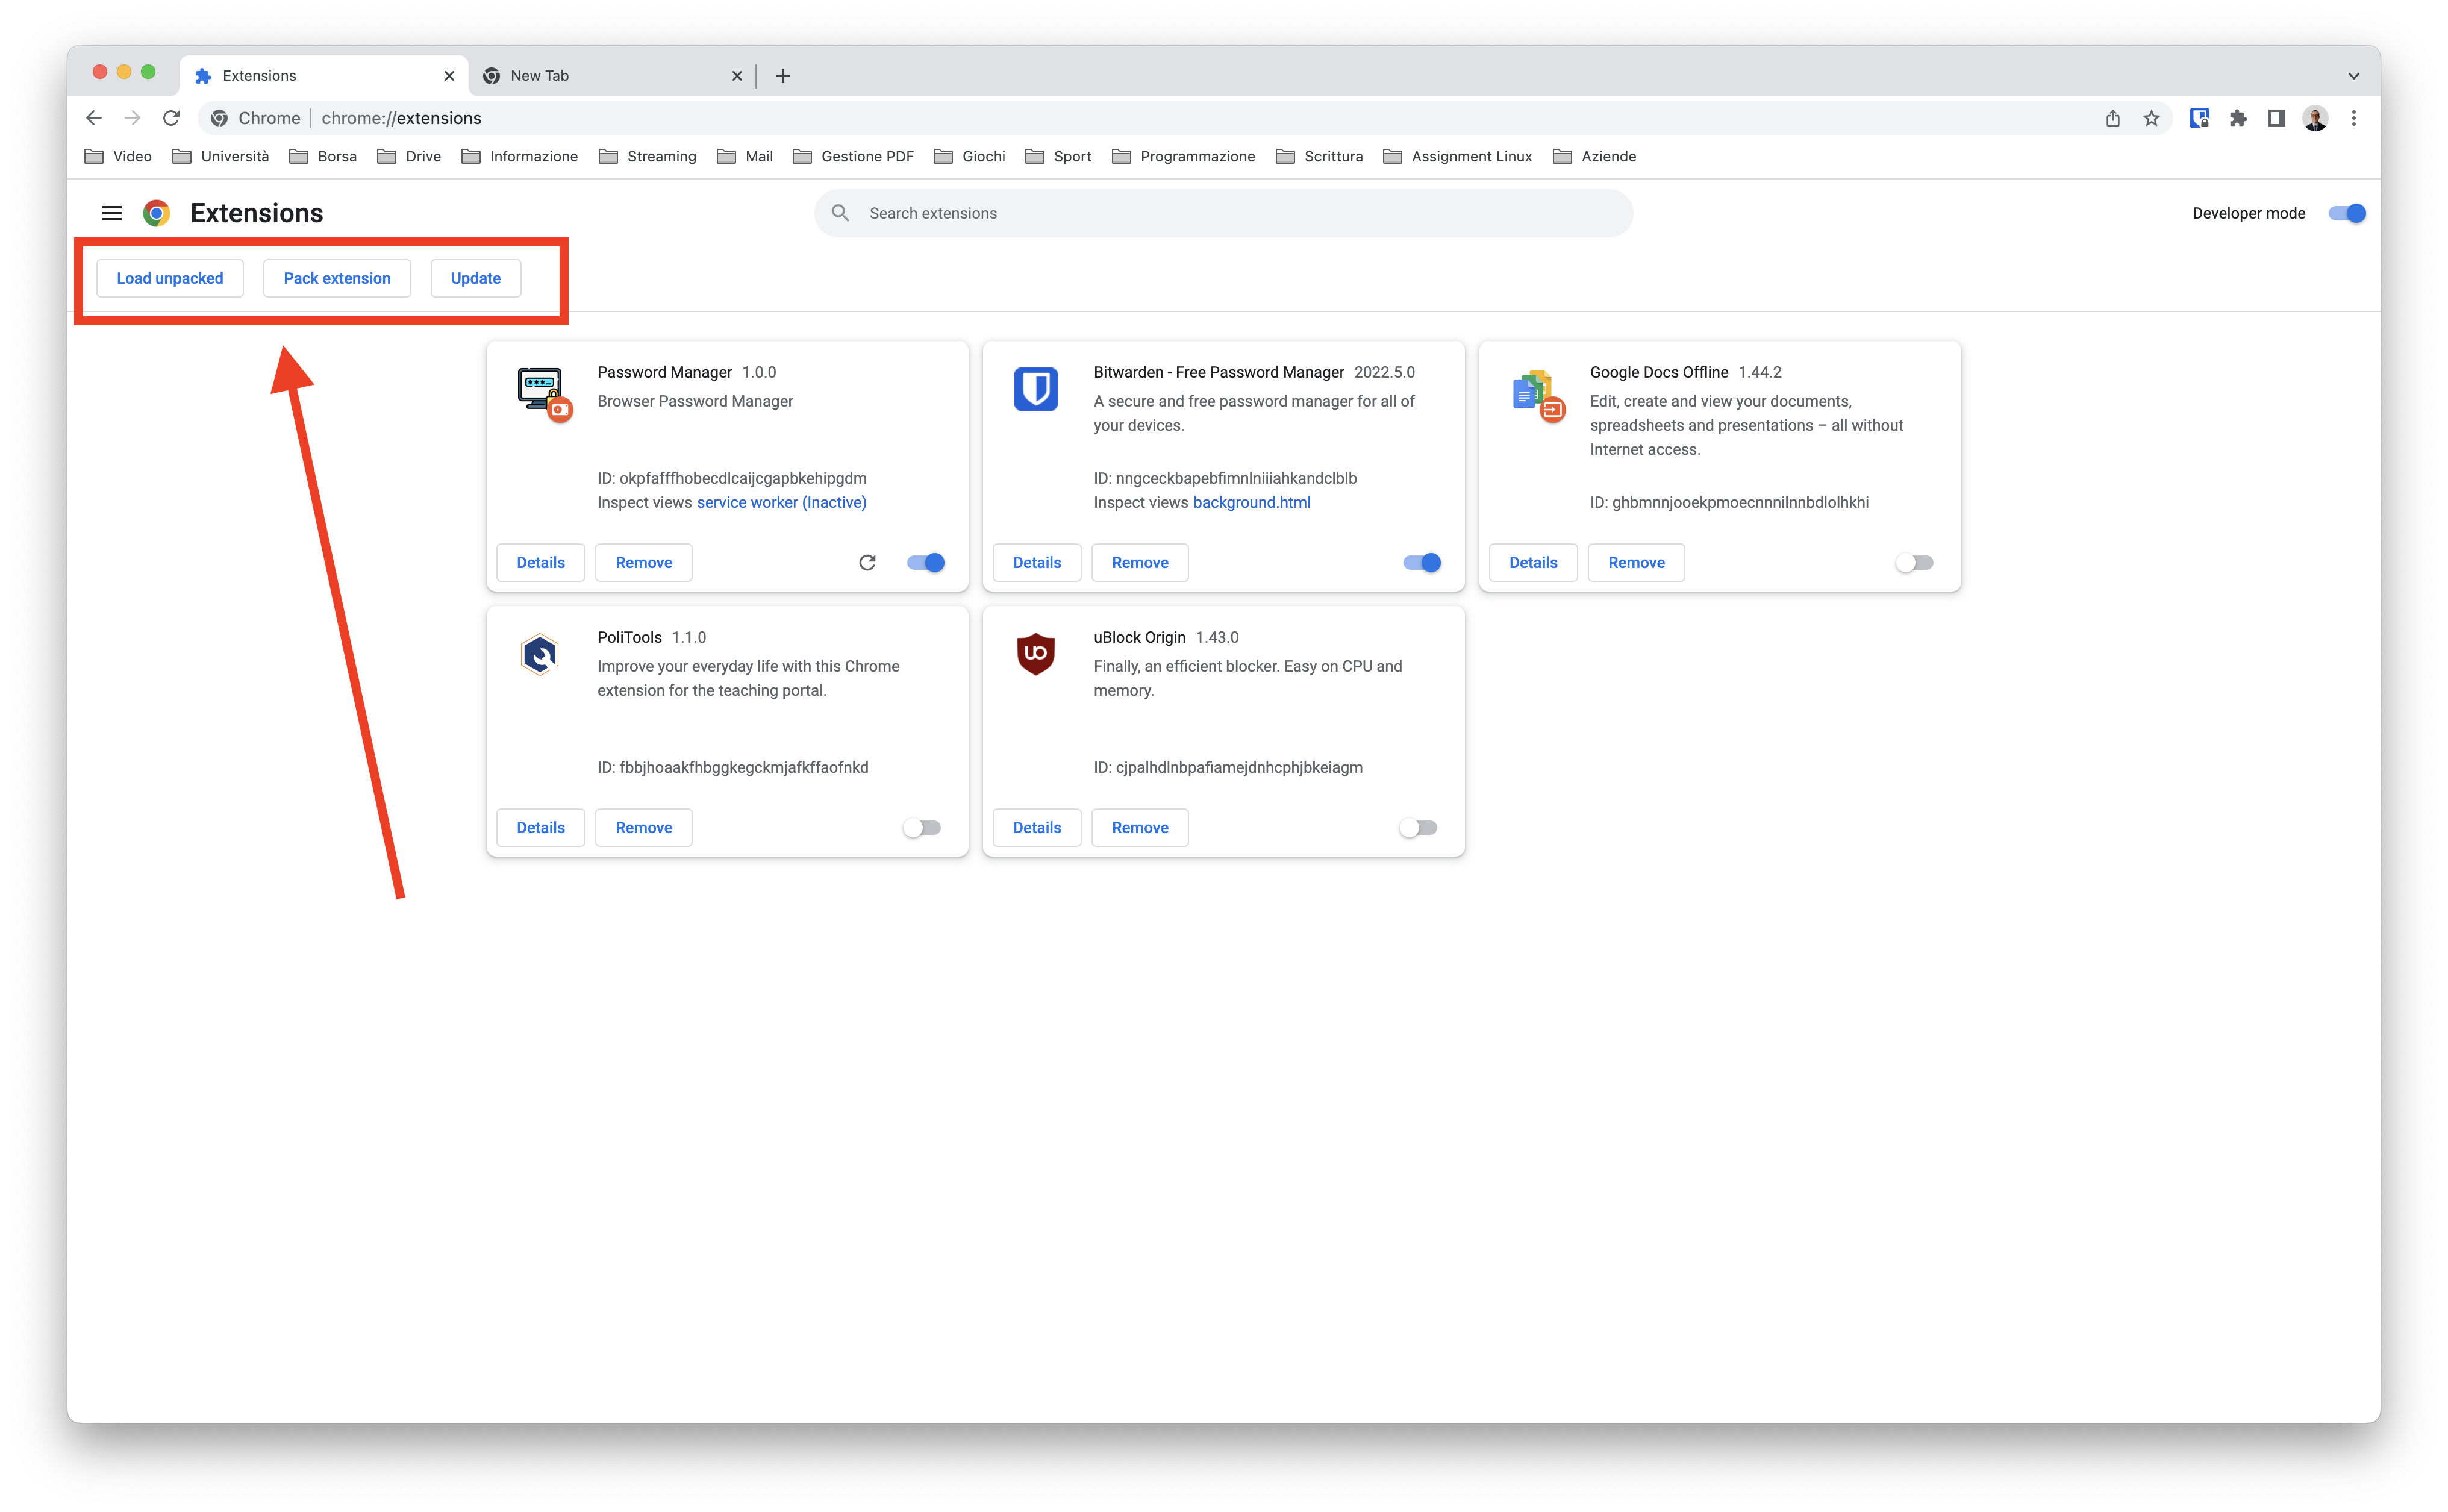
\includegraphics[width=0.8\textwidth]{images/extension/load-unpacked.png}
	\caption{Load Unpacked Extension}
	\label{fig:load_unpacked}
\end{figure}
The folder to be selected is the \texttt{dist} folder. 
\begin{figure}[htb]
	\centering
	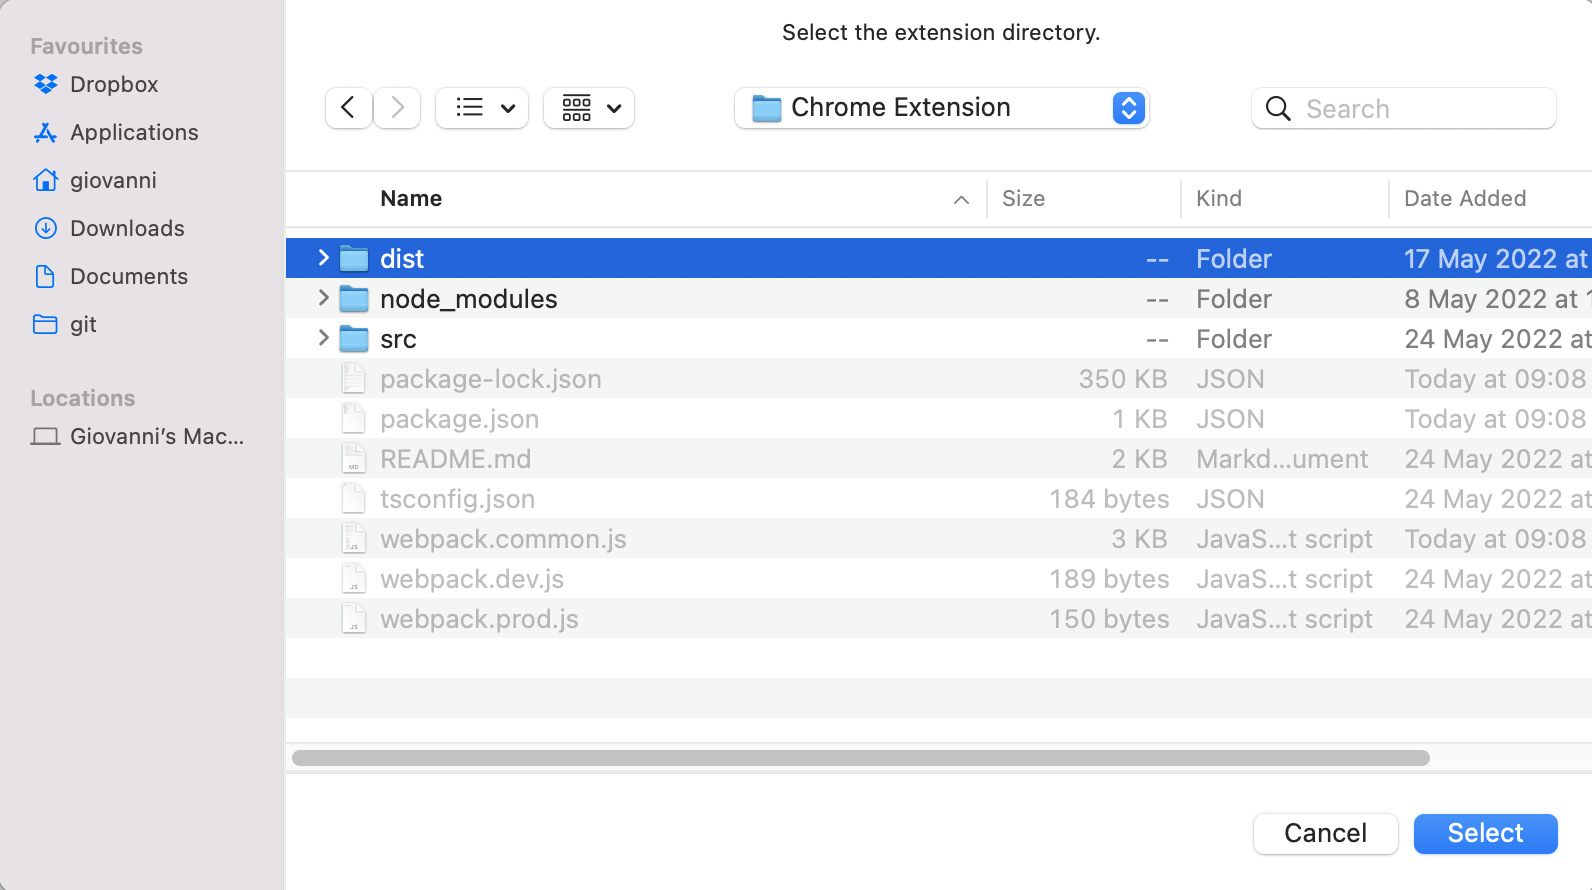
\includegraphics[width=0.8\textwidth]{images/extension/dist.png}
	\caption{Folder to load in the browser for the extension}
	\label{fig:dist}
\end{figure}

\subsubsection{Accepting the certificate}
\label{sec:accept_certificate}
The first time the extension is loaded into the browser, in order to use it, it is important to accept the certificate. In fact, when opening the popup, you will notice a message at the bottom. It says:

\begin{warning}
	Tesing version: if you are not able to login go to https://127.0.0.1:5000/ and accept the certificate
\end{warning}
By clicking the link a page like the one in the \autoref{fig:certificate1}  will appear. 

\begin{figure}[htb]
	\centering
	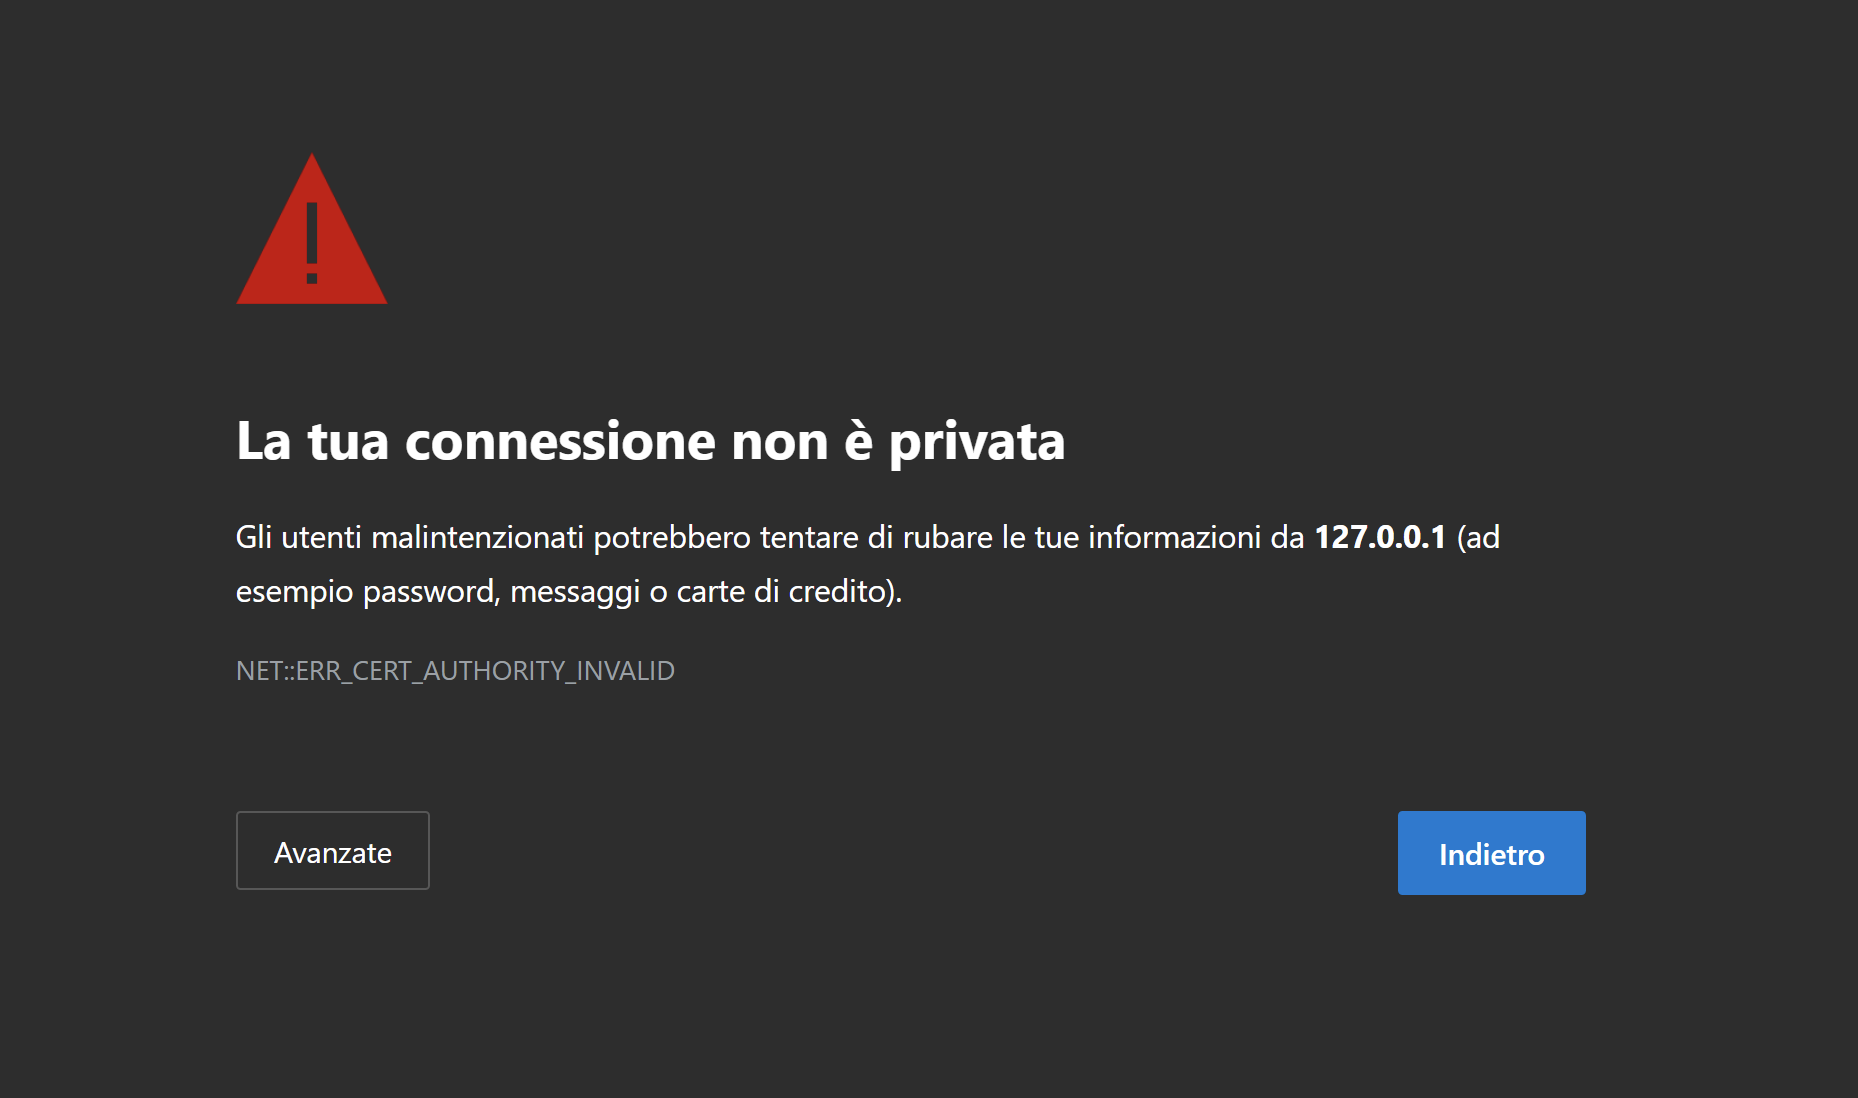
\includegraphics[width=0.8\textwidth]{images/extension/certificate1.png}
	\caption{Your connection is not private}
	\label{fig:certificate1}
\end{figure}
Here you just need to click on the \textbf{Avanzate} (Advanced in english) button. The page will expand as shown in the \autoref{fig:certificate2} below.
\begin{figure}[htb]
	\centering
	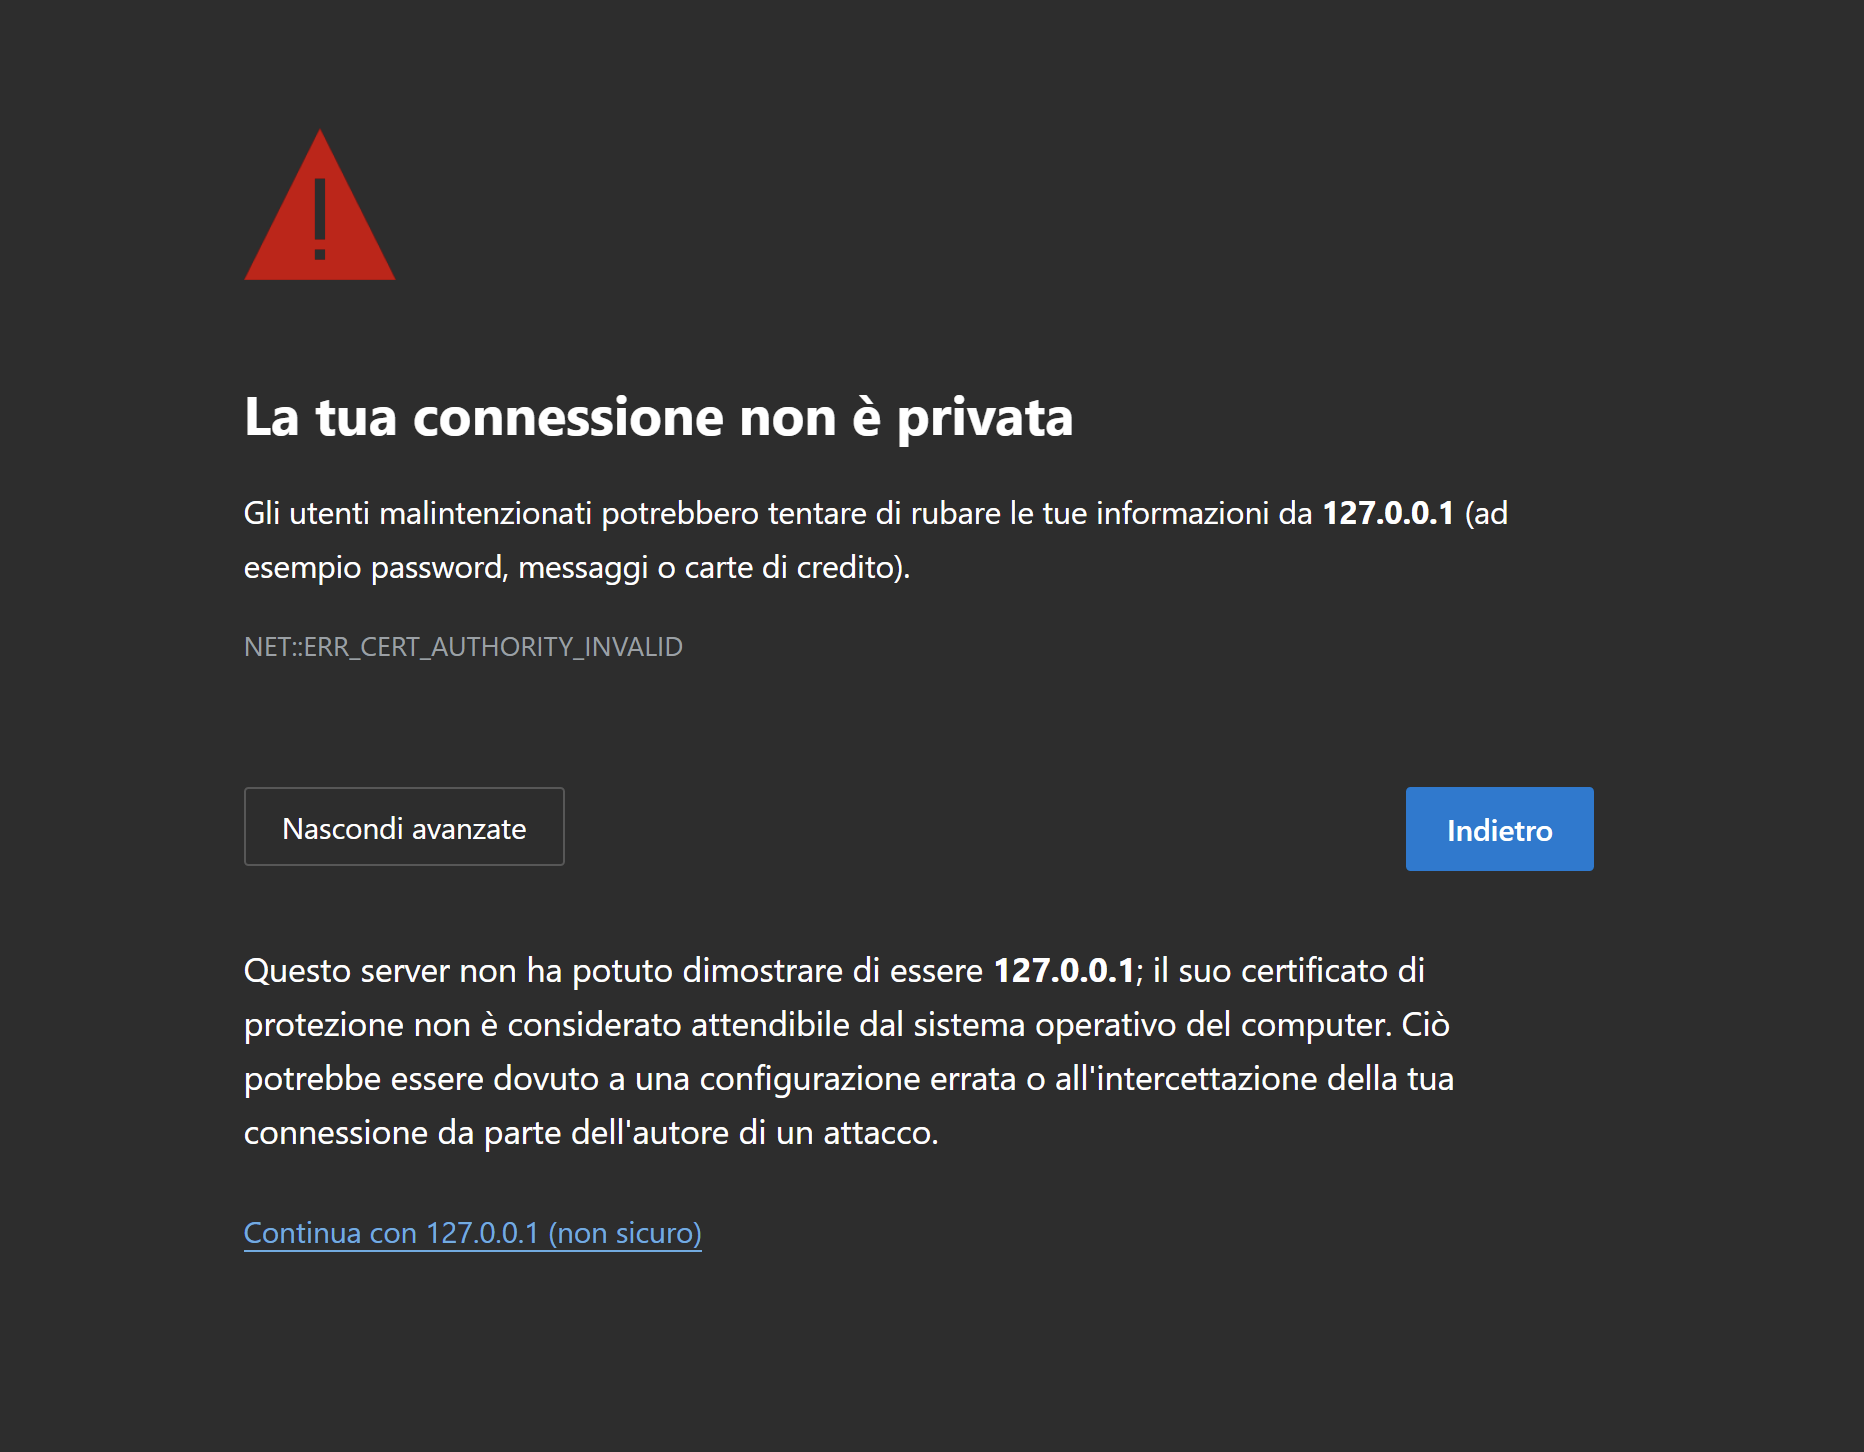
\includegraphics[width=0.8\textwidth]{images/extension/certificate2.png}
	\caption{Your connection is not private expanded}
	\label{fig:certificate2}
\end{figure}
Here you just need to click on the \textbf{Continua con 127.0.0.1 (non sicuro)} (Proceed to 127.0.0.1(unsafe) in english) button. The page shown in the \autoref{fig:certificate3} below will appear.
\begin{figure}[htb]
	\centering
	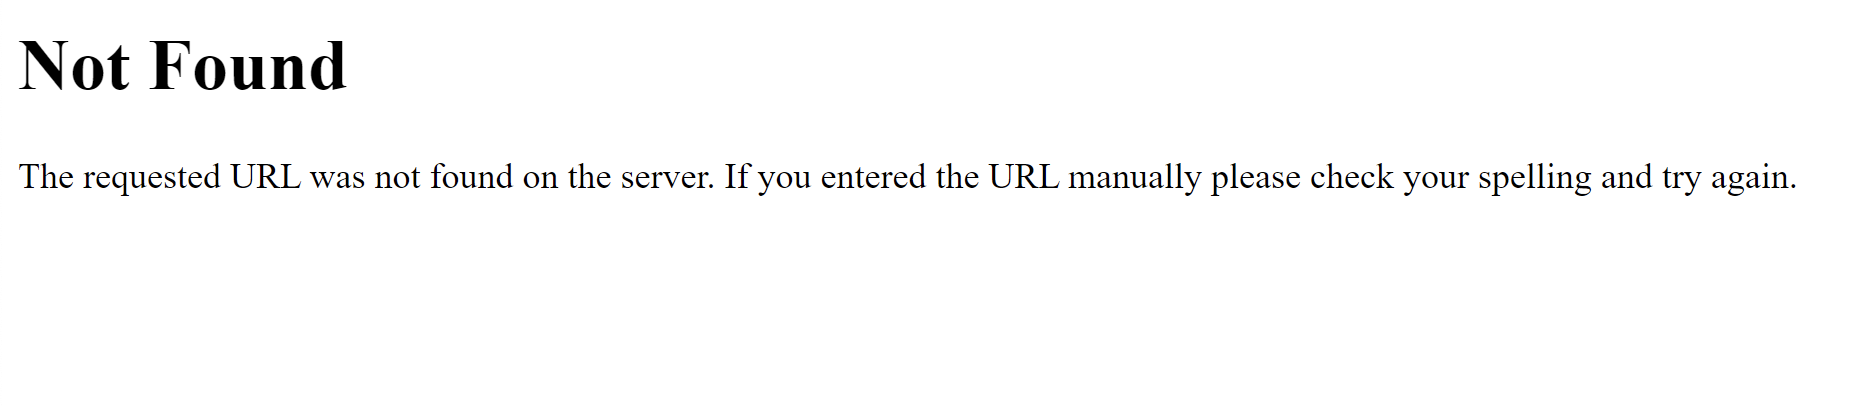
\includegraphics[width=0.7\textwidth]{images/extension/certificate3.png}
	\caption{Final page of the certificate process}
	\label{fig:certificate3}
\end{figure}
After all these steps you are ready to use the extension.


This steps will work on most of Chromium versions. However, in the newest the procedure may differ a bit. You will not find any \textbf{Advanced} button. To make it work you simply need to click in a blank part of the page a start typing \textbf{thisisunsafe}.

\begin{warning}
	\textbf{ATTENTION}: You will not have a visual feedback when typing, but the browser will accept it.
\end{warning}

After that the page will load the same page as the one shown in \autoref{fig:certificate3}